\chapter{Vorbetrachtungen}

\section{Softwareentwicklung}

In dieser Arbeit soll der Begriff Softwareentwicklung den Prozess benennen, der alle Aktivit"aten und die damit verbundenen (Zwischen-) Ergebnisse bei der Erstellung von Software umfasst.
In der Literatur wird auch der Begriff Softwareprozess genutzt \cite{Sommerville2001a}.
Obwohl es verschiedene Vorgehensmodelle f"ur das Erstellen von Software existieren, haben alle Softwareentwicklungsprozesse vier grundlegende Arbeitsaktivit"aten gemeinsam \cite{Brugge2004a,Sommerville2001a}:
\begin{description}
	\item[Softwarespezifikation:] Es m"ussen die konkreten Anforderungen an das zu erstellende Programm ermittelt werden.
								  Dabei wird die Funktion der Software, aber auch die Grenzen der Benutzung definiert.
	\item[Softwareentwurf und -implementierung:] Nach Analyse der ermittelten Anforderungen kann die Architektur des Softwaresystems entworfen werden.
												 Durch die Zerlegung der Software in mehrere Subsysteme werden die Anforderungen in kleine Teilprobleme aufgeteilt.
												 Diese Teilprobleme sind den verschiedenen Komponenten und Objekte der Software zugeordnet und k"onnen seperat gel"ost werden.
												 Diese L"osung wird durch die Objektentwurf und die schlu\ss endliche Implementierung erreicht.
	\item[Validierung der Software:] Die fertige Software muss auf ihre Funktionsf"ahigkeit "uberpr"uft werden.
									 Hierbei ist aber auch abzusichern, dass die Software neben der gew"unschten Funktionalit"at keine ungewollten Nebeneffekte (\emph{bugs}) auftreten.
	\item[Weiterentwicklung:] Ein Programm muss sich im Laufe seiner Lebenszeit weiter entwickeln um den sich "andernden Nutzeranforderungen gerecht zu werden.
\end{description}

\begin{figure}
\centering
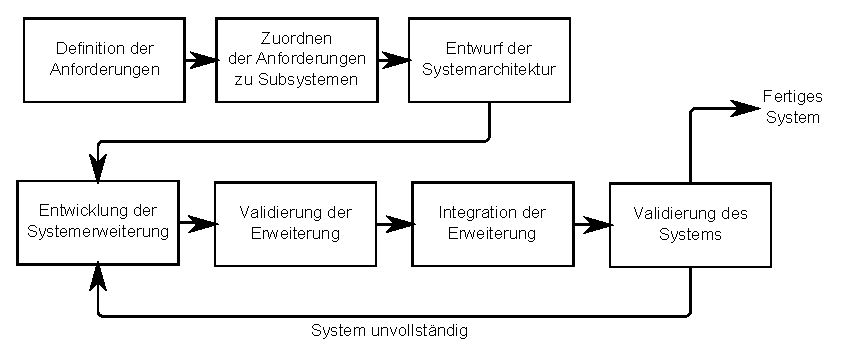
\includegraphics[width=\textwidth]{bilder/inkrementelle_entwicklung.eps}
\caption{Inkrementeller Softwareentwicklungsansatz nach \cite{Sommerville2001a}}
\label{pic:inkrementelle_entwicklung}
\end{figure}
F"ur die in dieser Arbeit zu entwickelnden Sofware wird die Methode der inkrementellen Entwicklung genutzt.
Die Herangehensweise dieser Methode ist in Abbildung \ref{pic:inkrementelle_entwicklung} dargestellt.
Nach der anf"anglichen Feststellung und Definition der grundlegenden Anforderungen an die zu programmierende Software, wird die allgemeine Struktur des Programms festgelegt.
Die Subkomponenten des Programms werden einzeln entworfen und in das bestehende Programm integriert.
Da die neuen Subkomponenten immer Teilanforderungen des Programmes erf"ullen, steigert sich somit die Funktionalit"at des Programms.
Dieser Ansatz hat den Vorteil, dass die Software schon zeitig im Entwicklungsstadium ausprobiert und getestet werden kann und damit auch schon Erfahrungen gesammelt werden k"onnen.
Zus"atzlich k"onnen gew"unschte "Anderungen der Bedienung oder der Funktionalit"at erkannt und implementiert werden.

Der letzte der vier oben genannten Aspekte ist in dieser Arbeit ein nicht zu vernachl"assigender Punkt.
Weil gerade das Programm f"ur die Nutzung w"ahrend der Entwicklung von Signalverarbeitungsmethoden erstellt wird, werden die Anforderungen an das Programm fortlaufend wachsen.
Somit soll schon von Beginn an die Erweiterbarkeit dieses Projektes unterst"utzt und gef"ordert werden.
Deshalb sind auch in den folgenden Anforderungen auch Punkte enthalten die diesen Aspekt besonders hervorheben und explizit fordern.

%Theorie zu Softwareentwurf
%-- Anforderungen: funktional und nichtfunktional
%-- Weiterentwicklung

\section{Anwendungsf"alle}

In diesem und dem folgendem Abschnitt soll die zu erstellende Software genauer spezifiziert werden.
Dazu soll zun"achst eine Liste von Anwendungsf"allen ausgearbeitet werden.
%Um eine Anforderungsliste an die zu erstellende Software ausarbeiten zu k"onnen, soll zun"achst eine Liste von Anwendungsf"allen ausgearbeitet werden.
Aus der Liste h"aufiger Arbeitsabl"aufe und typischer Aufgabenstellungen wird ersichtlich, was der Nutzer von der Software erwartet.
Mithilfe dieser Erwartungen k"onnen im Anschluss die funktionalen Anforderungen an das Programm formuliert und festgelegt werden.
% besonderheiten/merkmale der zu ueberpruefenden signale
% typische aufgabenstellungen
% haeufige arbeitsablaeufe

% enumerate auf a), b), usw aendern
\renewcommand{\theenumi}{\alph{enumi}}
\renewcommand{\labelenumi}{\theenumi )}
% und los geht's
Der Anwender m"ochte ...
\begin{enumerate}
	\item einen Datensatzes laden.
		  Dieser Datensatz umfasst mehrere (Bio-) Signale die sowohl mit einer konstanten Abtastrate erfasst wurden als auch Signale die nicht zu "aquidistanten Zeitpunkten abgetastet wurden.
	\item einen geladenen Datensatz mit allen "Anderungen speichern.
		  Hierbei sollen auch Einstellungen gespeichert werden, die die optische Pr"asentation wiederspiegeln.
	\item sich Informationen zu dem geladenen Datensatz und seinen beinhalteten Signalen anzeigen lassen und ver"andern.
	\item bestimmte Signale des Datensatzes ausw"ahlen und sich diese in ihrem Verlauf anzeigen lassen (Signalansicht).
		  Hierbei m"ochte er Bildschirmgr"o\ss e der einzelnen Ansichten ver"andern.
	\item die Signalansicht bez"uglich der Zeit- und der Amplitudenachse vergr"o\ss ern und verkleinern k"onnen (Zoomen).
		  Entlang der Zeitachse m"ochte er sie verschieben k"onnen (Scrollen).
		  Signaleverl"aufe die parallel aufgenommen wurden, sollen auch zusammen gescrollt werden.
	\item in einer Signalansicht mehrere Signale mit denselben Achsen darstellen lassen.
		  Beispielsweise um ein Roh- und ein verarbeitetes Signal miteinander vergleichen zu k"onnen.
	\item einen Amplitudenbereich eines Signals optisch hervorheben.
	\item einzelne Zeitpunkte im Signalverlauf mit einer Markierung versehen und kommentieren.
		  Diese Markierung kann sowohl f"ur ein bestimmtes Signal gelten, aber auch f"ur alle Signale des Datensatzes.
	\item einen Zeitabschnitt markieren. Die Markierung der Abschnitte soll analog zur Markierung von Zeitpunkten erfolgen.
	\item die Markierungen ver"andern (zeitlich verschieben, umbennen) oder l"oschen.
	\item Markierungen gemeinsam mit dem Datensatz aber auch unabh"angig vom Datensatz abspeichern.
\end{enumerate}

\section{Anforderungen}

Aus den oben genannten Anwendungsf"allen ergeben sich die folgenden Anforderungen an das Programm.
Das Programm ...
\renewcommand{\theenumi}{\Alph{enumi}}
\renewcommand{\labelenumi}{\theenumi )}
\newcommand{\AF}[1]{\item \label{AF:#1}}
\begin{enumerate}
	\AF{gui} muss eine grafische Benutzeroberfl"ache besitzen.
	\AF{datensatz} muss ein Datensatzformat unterst"utzen, das "aquidistant und nicht "aquidistante abgetastete Signale speichern kann.
	\AF{datenmanagement} soll in der Lage sein, Daten aus einem Datensatz zu laden.
						 Dem Nutzer muss es erm"oglicht werden, diese Signaldaten aus einer "Ubersicht auszuw"ahlen und in Diagrammen darstellen zu lassen.
						 Ferner muss der Benutzer eine M"oglichkeit haben, sich allgemeine Informationen des Datensatzes anzeigen zu lassen.
	\AF{diagramm} muss in der Lage sein, die Signalverl"aufe sowohl einzeln in einem Diagramm daszustellen, aber auch mehrere verschieden Signalverl"aufe in ein und demselben Diagramm zu visualisieren.
				  Diese Signalansichten sollten in ihrer Darstellungsgr"o\ss e durch den Nutzer ver"anderbar sein.
	\AF{ansicht} soll dem Benutzer erm"oglichen, seine Signalansicht frei "`bewegen"' zu k"onnen.
				 Es muss eine Vergr"o\ss erung und Verkleinerung bez"uglich der Abszissen- und der Ordinatenachse unterst"utzen.
				 Zus"atzlich ist die F"ahigkeit des Verschiebens der Ansicht gefordert.
				 Dabei sollen mehrere Diagramme gleichzeitig Verschoben werden k"onnen.
	\AF{amplitudenmarkierung} muss in der Lage sein einen Amplitudenbreich ein oder mehrerer Signalansichten optisch hervorzuheben.
	\AF{annotationen} soll dem Nutzer ein Werkzeug zur Verf"ugung stellen, das ihm erlaubt Datenpunkte zu annotieren.
					  Diese Annotationen sollen optisch in den Signalansichten ersichtlich sein und mit einem Kommentar versehen werden k"onnen.
					  Neben der Annotation einzelner Datenpunkte, soll auch die Markierung von Signalbereichen unterst"utzt werden.
					  Ferner ist gefordert, dass vorhandene Annotationen ver"anderbar sind.
	\AF{io} muss "Anderungen an den Signalen selbst und den Annotationen speichern k"onnen.
			Annotationen m"ussen unabh"angig von anderen Signalen gespeichert werden k"onnen.
			Insbesondere d"urfen Annotationen sich nicht ver"andern, wenn sich das Ursprungssignal ver"andert oder nicht mehr vorhanden ist.
	\AF{einstellungen} soll interne Einstellungen abspeichern und von einer Sitzung zur n"achsten "ubernehmen.
					   Optionen bez"uglich der Darstellung von Signalen sollen in dem Datensatz mit abgespeichert werden k"onnen.
\end{enumerate}

Die in der Aufgabenstellung geforderte Ausbauf"ahigkeit der Programms kann nicht durch die Anwendungsf"alle abgedeckt werden.
Hierbei handelt es sich um eine nichtfunktionale Anforderung an das Programm.
Daher wird die folgenden Anforderung nur auf Basis der Aufgabenstellung formuliert und nicht aufgrund der Erwartungshaltung des Benutzers:
%Die folgende Anforderung l"asst sich nicht aus den Anwendungsf"allen erschlie\ss en, das die Erweiterbarkeit eine Forderung von zuk"unftigen Entwicklern ist und nicht die der Anwender.
%Um aber die Ausbauf"ahigkeit des Programms zu erm"oglichen, muss es 
\begin{enumerate}[resume]
	\AF{signalverarbeitung} Das Programm soll dem Benutzer erm"oglichen eine Signalverarbeitungsmethode auf ein gew"ahltes Biosignal anwenden zu k"onnen.
							Dabei muss das Originalsignal unver"andert bleiben.
							Der bearbeitete Signalverlauf kann als eigenes Signal im Datensatz abgespeichert werden.
							Die Implementierung dieser Anforderung soll beispielhaft f"ur zuk"unftige Entwickler erfolgen um die Erweiterbarkeit zu gew"ahrleisten.
\end{enumerate}

\section{Testszenarien}

-- Implementierung und Fehlerbehebung
-- konstant fortlaufender prozess
-- komponenten test hier nicht abgebildet und beschrieben - sind schon durch inkrementelle entweicklung gef"ordert
-- Validierung

In der Softwareentwickluin

Um das Programm auf seine Funktionsf"ahigkeit zu "uberpr"ufen sollen in diesem Abschnitt Tests ausgearbeitet werden.
Sie erm"oglihcen es das Progrmam zu testen und auf seine funktionf"ahigkeit zu "uberpr"ufen.
Daher brauchen wir ein paar Testszenarien f"ur die FUnktionspr"ufung des F"ahigkeits"uberpr"ufungsroutinendingens.

% Szenarien aus der Anforderungsliste abgeleitet

%% EOF %%%%%%%%%%%%%%%%%%%%%%%%%%%%%%%%%%%%%%%%%%%%%%%%%%%%%%
